\section{Vector Space Retrieval Model: Simplest Instantiation}

\subsection{What VSM Doesn’t Say}
\begin{figure}[H]
    \centering
    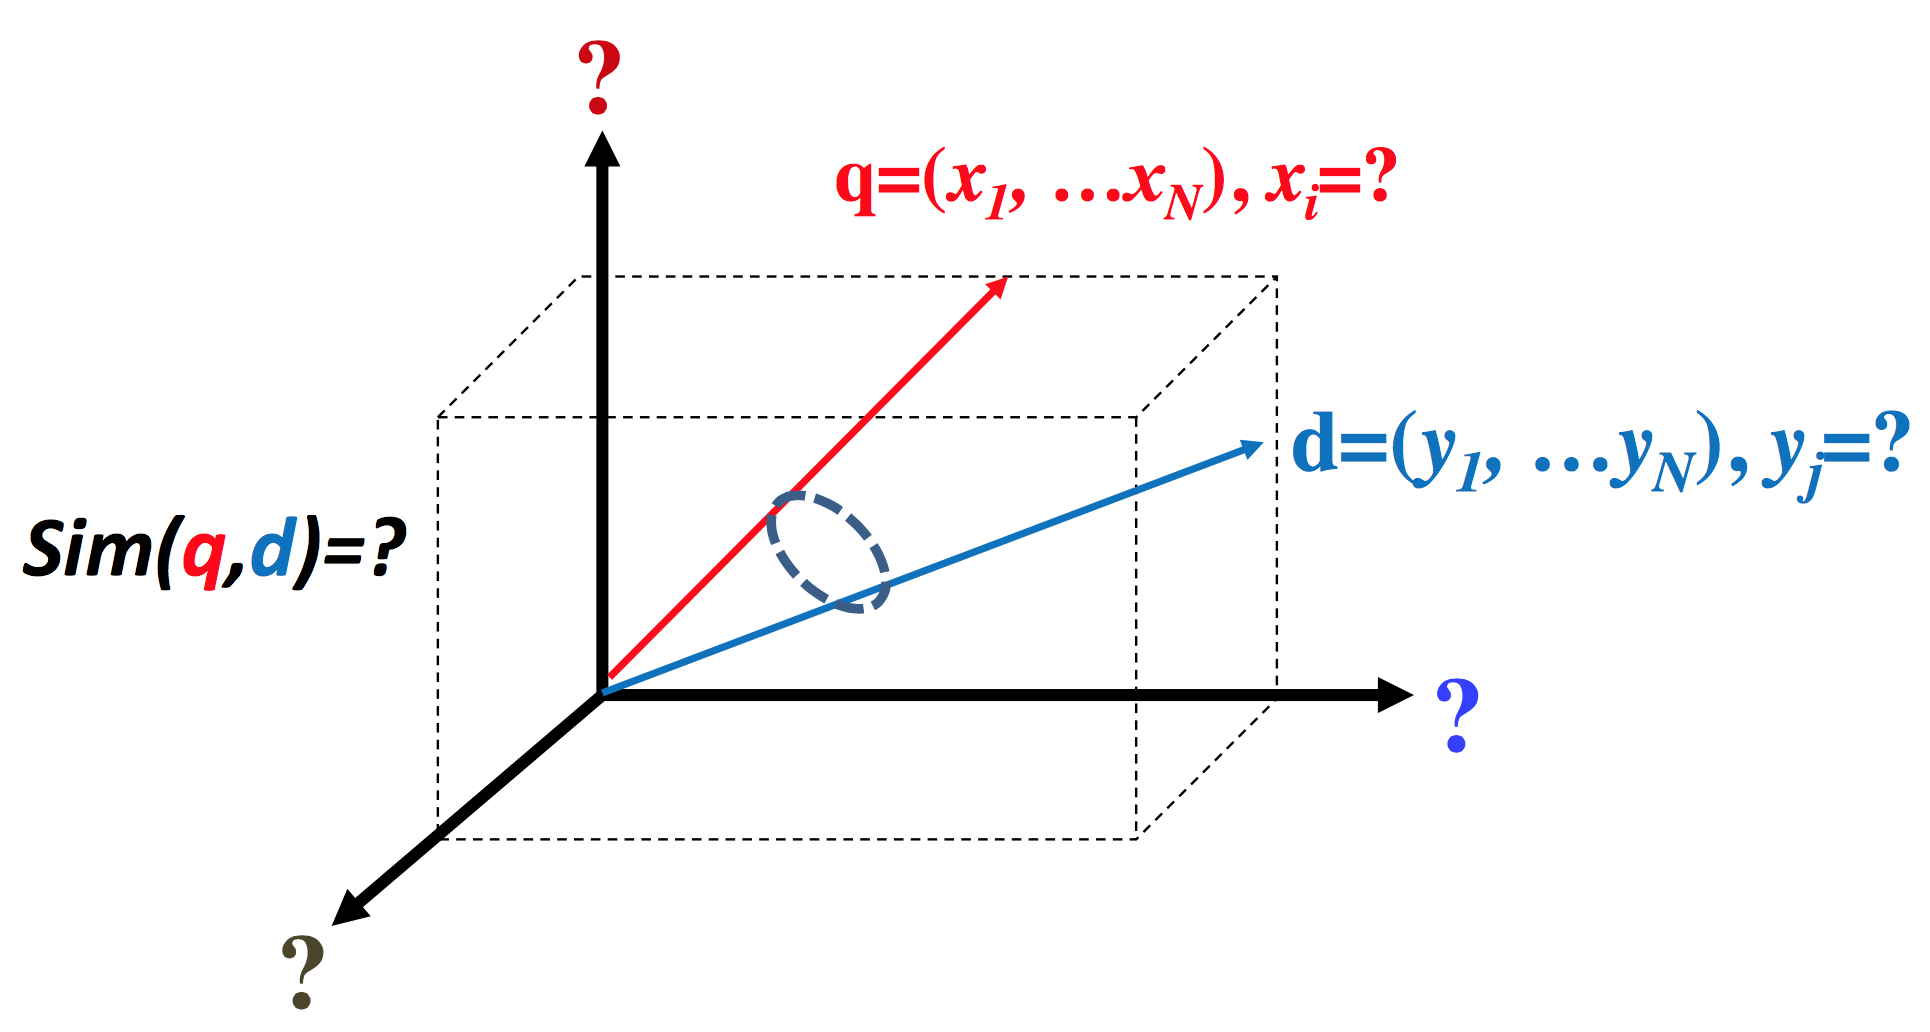
\includegraphics[width=\linewidth]{vsm_questions.png}
\end{figure}



\subsection{Simplest VSM= Bit-Vector + Dot-Product + BOW}
\begin{figure}[H]
    \centering
    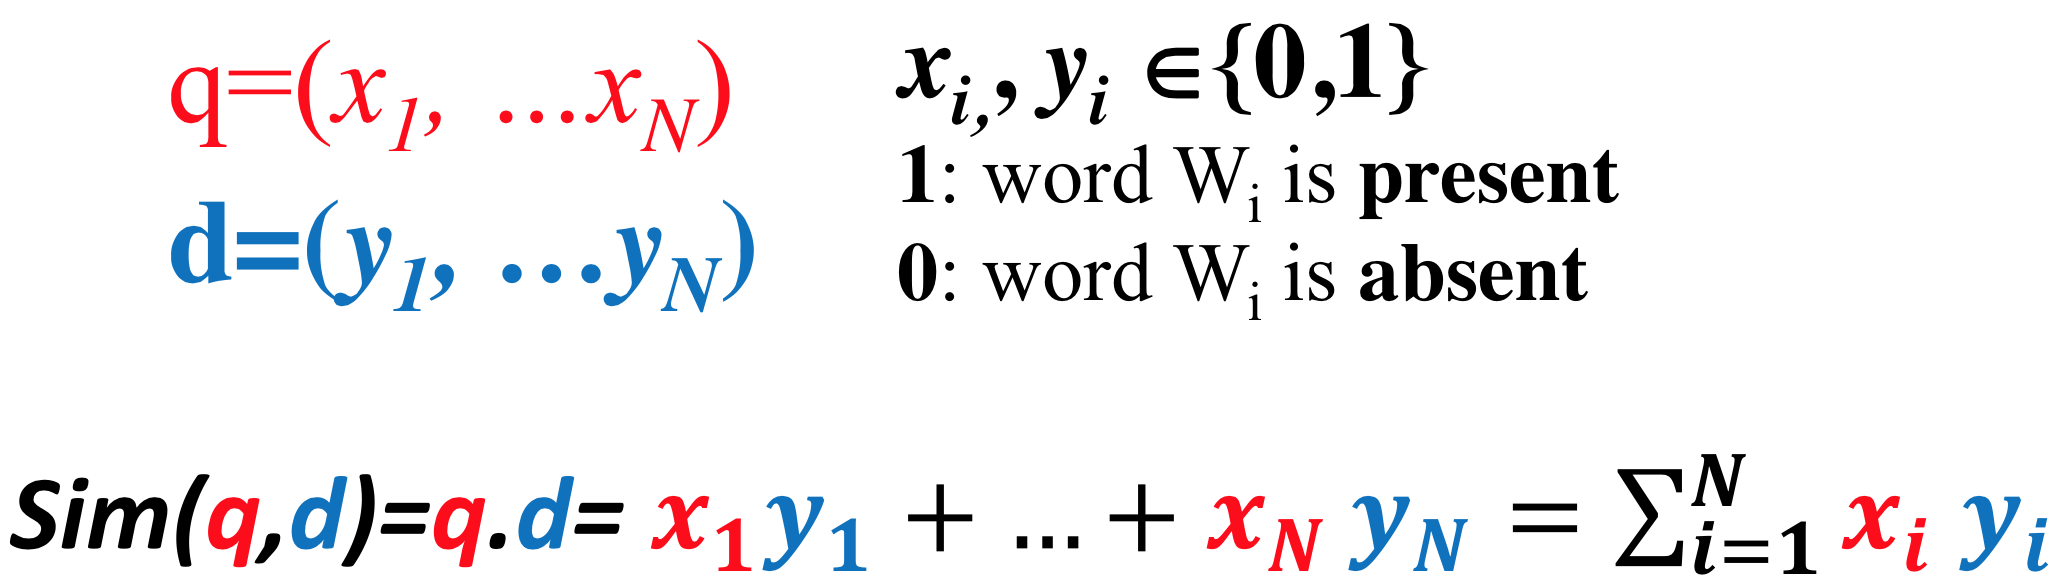
\includegraphics[width=\linewidth]{simplest_vsm.png}
\end{figure}

Simplest VSM:
\begin{itemize}
\item Dimension = word
\item Vector = 0-1 bit vector (word presence/absence)
\item Similarity = dot product
\item f(q,d) = number of distinct query words matched in d
\end{itemize}
